\begin{figure*}[ht]
    \centering
    \begin{subfigure}[t]{0.47\textwidth}
        \centering
        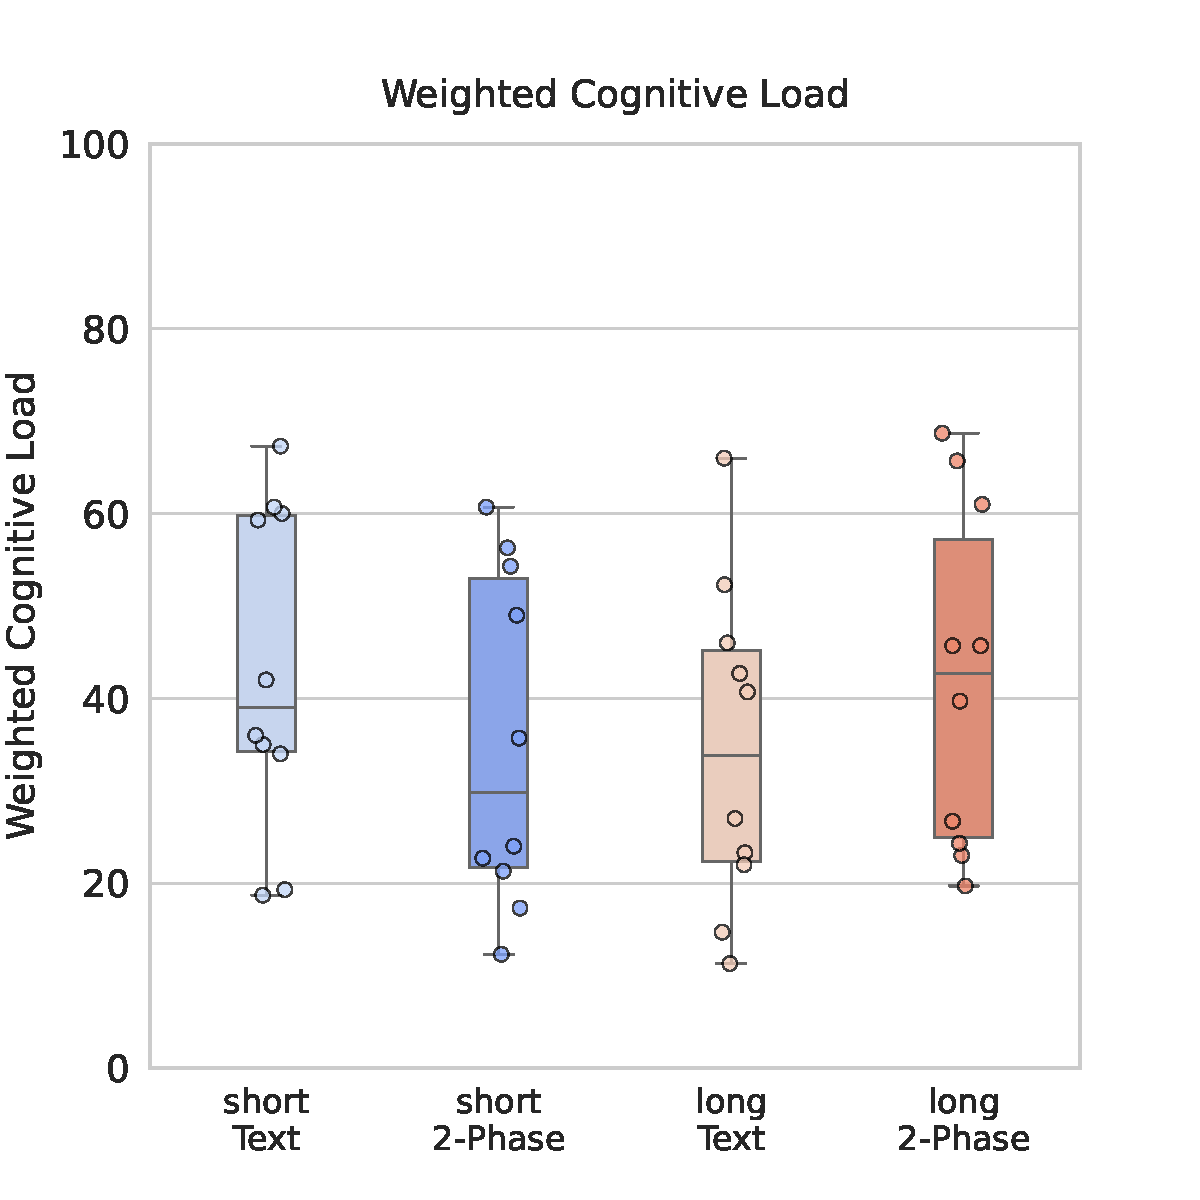
\includegraphics[width=0.95\textwidth]{content/image/results/nasatlx_final_value.pdf}
        \caption{NASA-TLX Weight Score: The Long Two-Phase Interface exhibits the highest weighted cognitive load with a median of $42.70$, a mean of $42.02$. This is higher than the long text interface, which has a median cognitive load of $33.85$ and a mean of $34.60$. However, the short text interface demonstrates a higher cognitive load with a median of $39.00$, a mean of $43.23$, compared to the short two-phase interface, which has a median of $29.85$, a mean of $35.36$. The standard deviation is similar across groups at around $18$.}
        \Description{A box plot comparing weighted cognitive load scores across four interface conditions: short text, short two-phase, long text, and long two-phase. The y-axis is labeled "Weighted Cognitive Load" and ranges from 0 to 100. Each condition is represented by a box with whiskers, and individual data points are plotted as circles. The short text and long two-phase interfaces show higher cognitive load distributions, while the short two-phase and long text interfaces show lower distributions. The title reads "Weighted Cognitive Load."}
        \label{fig:nasatlx-final1}
    \end{subfigure}
    \hfill
    \begin{subfigure}[t]{0.49\textwidth}
        \centering
        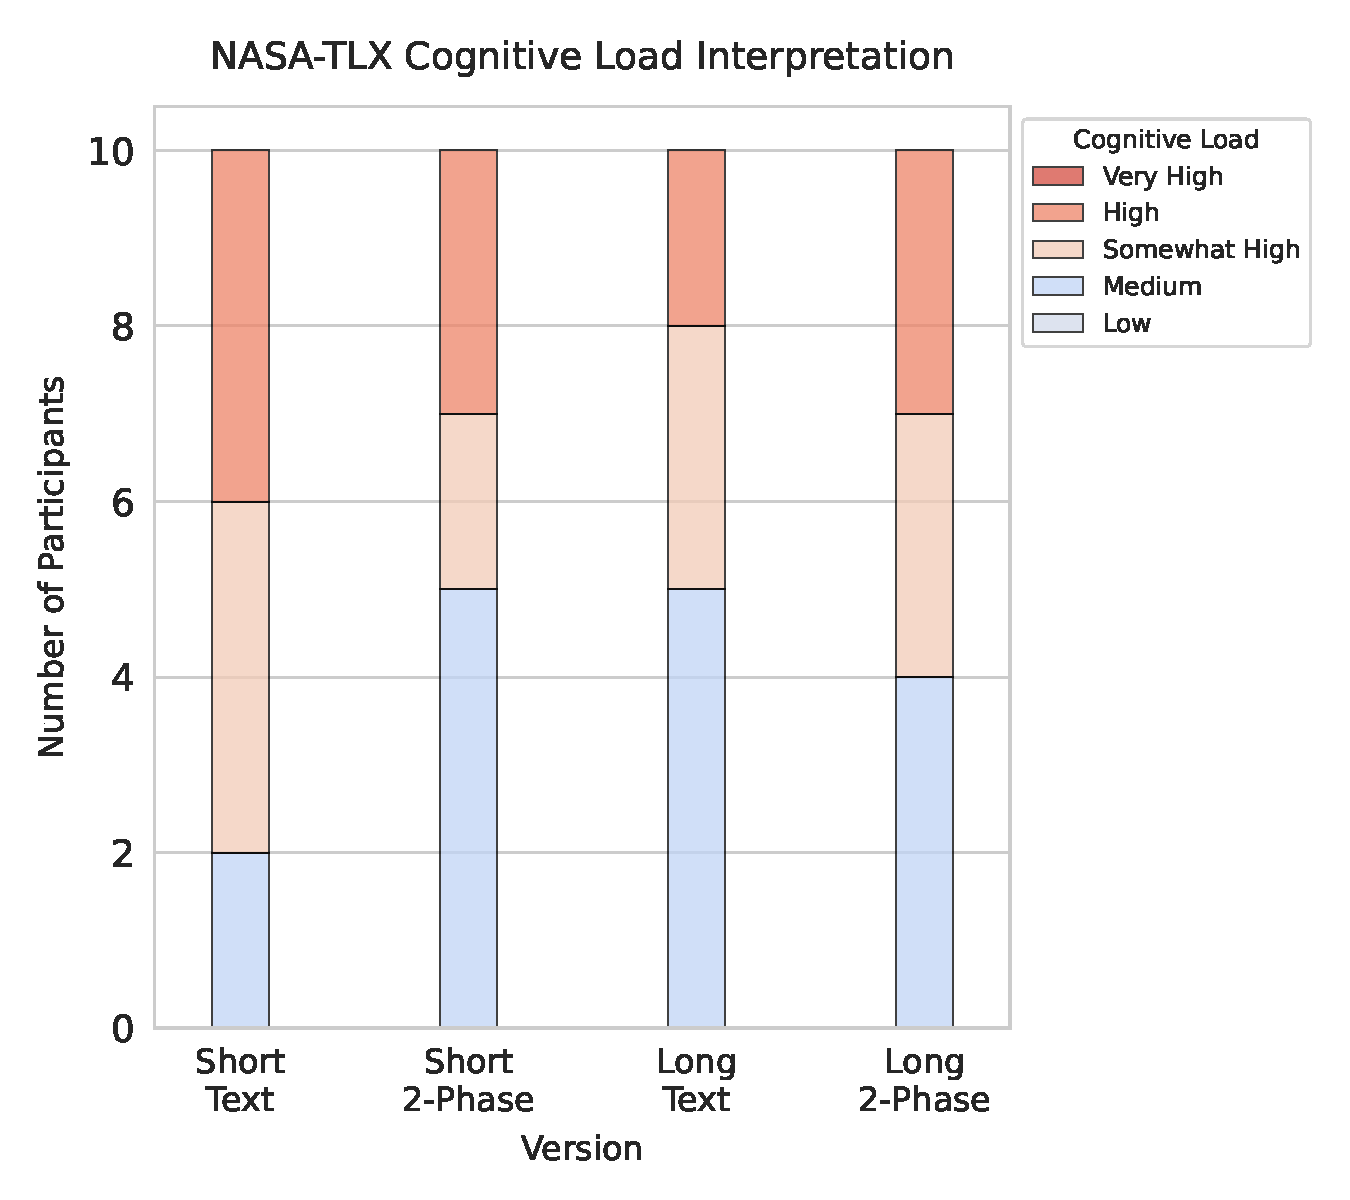
\includegraphics[width=1\textwidth]{content/image/results/nasatlx_cog_value_interpreted.pdf}
        \caption{NASA-TLX Cognitive Interpretation: More participants in the short text interface, totaling $8$, reported a somewhat high or above cognitive load, which is significantly higher compared to the $5$ participants who reported similarly for the short two-phase interface. However, the long two-phase interface saw slightly more participants, $6$ in total, reporting somewhat high or above cognitive load compared to the long text interface.}
        \Description{Stacked bar chart showing the number of participants experiencing different levels of cognitive load across four interface versions: Short Text, Short 2-Phase, Long Text, and Long 2-Phase. The y-axis represents the number of participants (from 0 to 10), and the legend differentiates five cognitive load levels: Low, Medium, Somewhat High, High, and Very High. The chart highlights more participants reporting higher cognitive loads for short text-based interfaces.}
        \label{fig:nasatlx-final2}
    \end{subfigure}
    \caption{This figure shows the box plot results for weighted NASA-TLX scores across experiment groups and participant counts based on individual score interpretations. In~\ref{fig:nasatlx-final1}, we observe a downward trend in cognitive load for the short QS, while the long QS shows an upward trend. Interestingly, there is a counterintuitive downward trend between short and long text interfaces. In~\ref{fig:nasatlx-final2}, these trends are clearer when NASA-TLX scores are grouped into five tiers.}
    \Description{Two figures side by side, a box plot to the left and a stacked bar chart to the right, representing the weighted NASA-TLX distributions and the interpretations respectively.}
    \label{fig:nasatlx-final}
\end{figure*}

\section{Result: Self-Reported Cognitive Load in Quadratic Surveys}
\label{sec:cog}
This section presents findings on cognitive load in QSs, focusing on how the number of options and different interfaces influence it (\textbf{RQ1}, \textbf{RQ2a}). We analyze similarities and differences in cognitive load sources across conditions (\textbf{RQ2b}).

Qualitative findings are based on an inductive thematic analysis~\cite{olsonWaysKnowingHCI2014}, which was conducted after transcribing the interviews. The first author single-coded the snippets according to the research questions and merged them into overarching themes. The first author conducted multiple rounds of coding, and identified differences across conditions, which were refined and validated using a deductive coding process.

Quantitative findings are derived from a Bayesian approach, which enhances transparency by interpreting posterior distributions and moving beyond binary thresholds~\cite{kay2016researcher}. Bayesian methods suit various sample sizes, leveraging maximum entropy priors to ensure conservative and robust inferences~\cite{mcelreath2018statistical}.

\subsection{Overall Cognitive Load from NASA-TLX}
\label{sec:cog_overall}
Weighted NASA-TLX uses a continuous $0$ to $100$ score, with higher values denoting greater cognitive load. We use predefined mappings of NASA-TLX scores to cognitive levels: low, medium, somewhat high, high, and very high, as described by~\citet{hart1988development}. Results are shown in Figure~\ref{fig:nasatlx-final1}, with value interpretations presented in Figure~\ref{fig:nasatlx-final2}.

Given the sparsity of the data, we modeled the weighted NASA-TLX scores as ordinal outcomes based on value interpretations. We developed a hierarchical Bayesian ordinal regression model with length as an ordinal predictor and interface type as a categorical predictor, using hierarchical priors for partial pooling. Interaction effects between length and interface are captured via a non-centered parameterization with an LKJ prior to account for correlations~\cite{mcelreath2018statistical}. We applied the same model to the NASA-TLX subscales; since these subscales lack inherent cognitive level interpretations, we constructed weighted bins for the ordinal regression. In our model, a latent variable represents a continuous measure of cognitive load, discretized into ordinal outcomes via thresholds. Details of this model and additional subscale results are provided in Appendix~\ref{apdx:model_tlx}.

\begin{figure*}[ht]
    \centering
    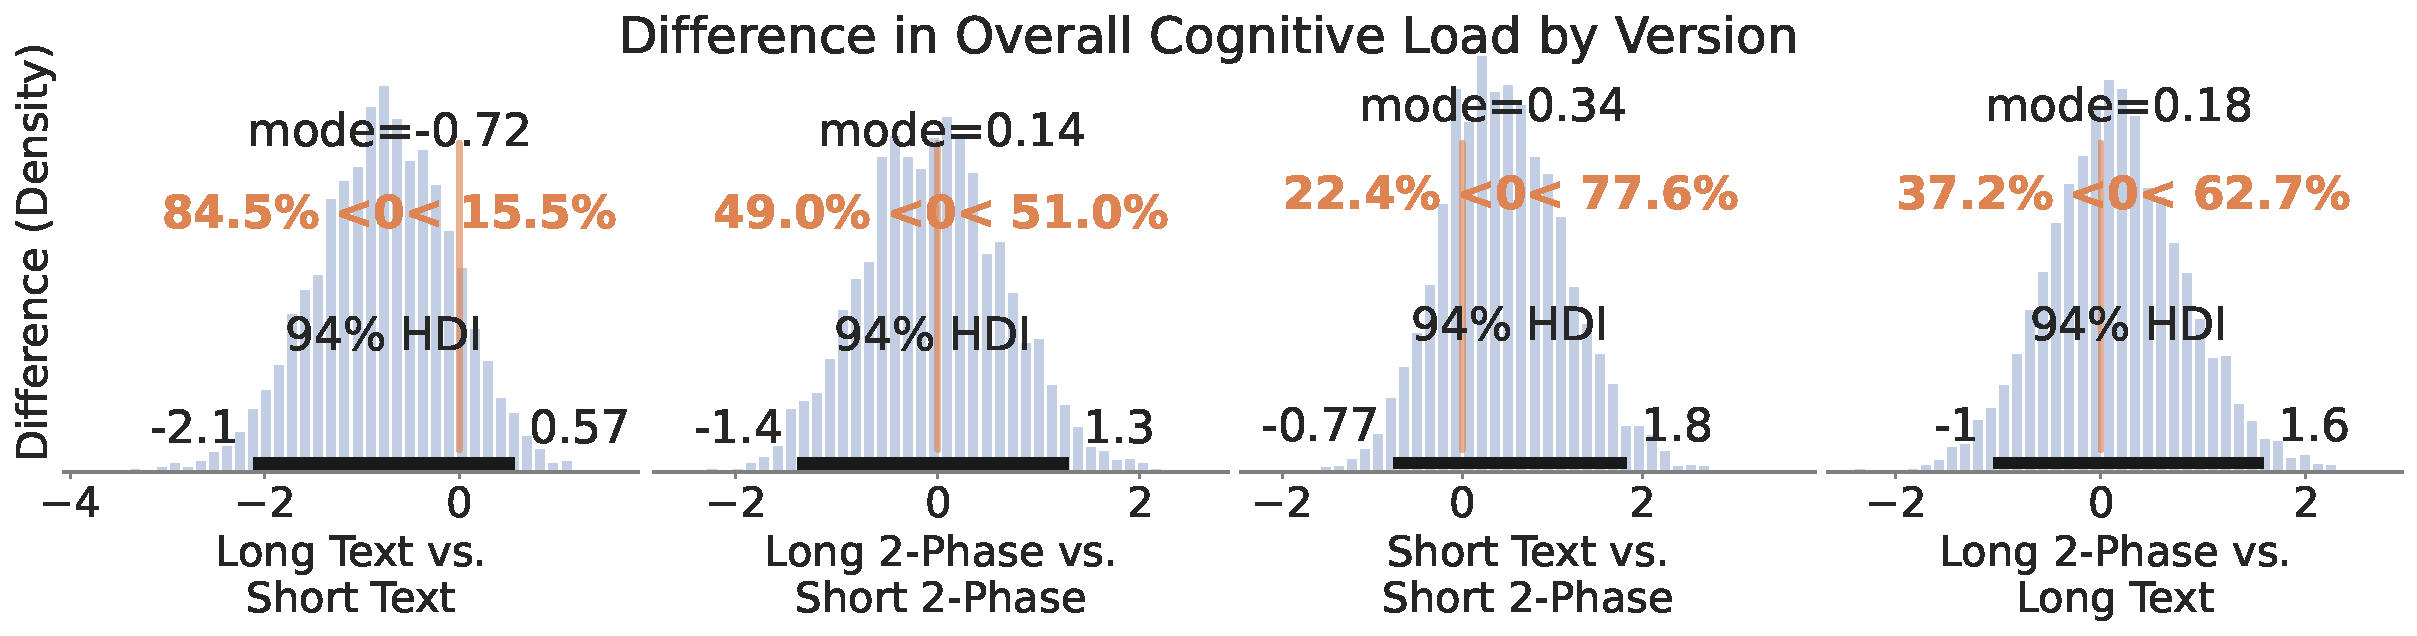
\includegraphics[width=0.8\textwidth]{content/image/cog/weighted_cog_version_single_row.pdf}
    \caption{Posterior distributions of differences in latent cognitive load between experimental conditions. Values below 0 indicate reduced load.~\textbf{Main takeaway:} while the model does not indicate statistically significant differences, longer text interfaces are more likely to reduce cognitive load, and the two-phase interface has a higher probability of lowering cognitive load.}
    \Description{A grouped panel of four histograms titled "Difference in Overall Cognitive Load by Version," displaying posterior distributions of differences between experimental conditions. Each plot shows density (y-axis) against the difference (x-axis) with summarized statistics. None of the orange lines are outside of the interval. Each histogram features a density curve with credible intervals, a vertical reference line at zero, and key values in orange. These values emphasize the distribution characteristics and differences across versions.}
    \label{fig:weighted_cog_version}
\end{figure*}

In Bayesian analysis, the 94\% high-density interval (HDI) represents the range where the true parameter is most likely to lie. While the results (Figure~\ref{fig:weighted_cog_version}) in terms of differences in latent cognitive load are not statistically significant because 0 is within this range, the HDI quantifies probabilistic trends and accounts for uncertainty in a transparent manner.
\begin{itemize}[leftmargin=*]
    \item Increased option length with text interface trends to~\textit{reduced} cognitive load with a posterior probability of approximately $84.5\%$. This reflects a median cognitive load of $33.85$ (mean = $34.60$, SD = $17.69$) compared to a median of $39.00$ (mean = $43.23$, SD = $17.65$).
    \item Within short QSs, the two-phase interface trends to~\textit{reduced} cognitive load, with a posterior probability of $77.6\%$ supporting the reduction. Participants report a median cognitive load of $29.85$ (mean = $35.36$, SD = $18.17$) under the two-phase interface compared to a median of $39.00$ (mean = $43.23$, SD = $17.65$) under the text interface.
    \item For the long QSs, the two-phase interface trends an~\textit{increase} in cognitive load with a posterior probability of $62.7\%$. The median cognitive load is $42.70$ (mean = $42.02$, SD = $18.48$) under the two-phase interface compared to $33.85$ (mean = $34.60$, SD = $17.69$) in the text interface.
\end{itemize}

This result contradicts our hypothesis that more options would increase cognitive load and that interfaces can reduce it. Thus, we explore qualitative results to identify possible explanations. To understand the similarities and differences in sources of cognitive load (\textbf{RQ2b}), we analyze qualitative results across the six NASA-TLX subscales: mental demand, physical demand, temporal demand, effort, frustration, and performance. Detailed breakdown of each subscale are provided in Appendix~\ref{apdx:cog_qual}.

\subsection{Qualitative Analysis: Common Sources of Cognitive Load}
\label{sec:cog_common}
Our analysis reveals several themes across different cognitive load subscales. We focus on three themes common to all experimental conditions, omitting less related themes for clarity.

\textbf{Preference Construction} is cited by 97.5\% (N=39) of participants as a significant source of mental demand, consistent with prior literature suggesting that preferences are often constructed in context rather than fixed~\cite{lichtensteinConstructionPreference2006}. Specific tasks contributing to this demand include evaluating the relative importance between options (e.g.,\smallquote{S002}{Figuring out\bracketellipsis how much I prioritize option 1 over option 2}, 40\% (N=16)), making trade-offs due to limited resources (e.g.,\smallquote{S005}{\bracketellipsis very hard to take decisions~\ldots I felt that multiple options deserve equal amounts of credit~\ldots but you have given very limited credit.}, 42.5\% (N=17)), and deciding the exact number of votes (e.g.,\smallquote{S023}{\bracketellipsis having to pick how many upvotes would go to each one}, 70\% (N=30)).

\textbf{Budget Management} emerges as a source of both mental and temporal demand. 25\% (N=10) of participants describe the challenge of working with limited credits while trying to maximize their allocation (e.g.,~\smallquote{S032}{~\bracketellipsis for certain societal issues, you had to~\ldots take away from other issues you could support}). An equal percentage of participants find it mentally taxing to keep track of remaining credits (e.g.,~\smallquote{S006}{~\bracketellipsis looking at the remaining credits, I'm trying to mentally divide that up before I start allocating}).

When assessing themes across all subscales, we identified patterns that highlights the underlying nature of participants' cognitive efforts across different contexts. Thus, we also coded interview snippets as~\textbf{Operational} and~\textbf{Strategic} actions in addition to goal-oriented actions such as Budget Management and Preference Construction.

\textbf{Operational Actions} refer to reactive efforts addressing immediate, tactical needs, which emerged across all experimental conditions. These actions involve direct task execution, responding to constraints without reflection on broader, long-term implications. Examples include adjusting choices to stay within budget (e.g.,~\smallquote{S003}{I had to alter~\bracketellipsis I kept going under budget}), re-reading options (e.g.,~\smallquote{S010}{I just had to reread it again}), completing questions efficiently (e.g.,~\smallquote{S010}{I was trying to be efficient in responding to the question}), and interacting with the survey interface (e.g.,~\smallquote{S018}{Like (deciding) one upvote or two upvotes\bracketellipsis}). 40\% (N=16) of participants attribute Operational actions to temporal demand. Additionally, 37.5\% (N=15) attribute this cause to frustration, and 32.5\% (N=13) attribute it to performance. While commonly cited across conditions, its distribution varies.

\subsection{Qualitative Analysis: Different Sources of Cognitive Load}
\label{sec:cog_diff}
There are several notable differences between the text and two-phase interfaces. 

First, regardless of length, when analyzing performance, which refers to a person's perception of their success in completing a task, participants describe their performances differently. We categorize them into indications of satisficing behaviors(``good enough''), exhausting their effort (i.e., ``done their best,''), or feeling positive (i.e., ``feeling good.'') There are almost twice as many participants using the two-phase interface to report a positive feeling about their final submission~(55\% v.s 30\% (N=11 vs. 6)).

Second, 70\% (N=14) of text interface participants attribute operational actions as contributors to effort, double the percentage observed in the two-phase interface group (35\%, N=7). This partially echoes the finding that 90\% (N=18) of text interface participants report mental demand from deciding the exact number of votes, compared to 60\% (N=12) in the two-phase interface group.

The distinction between the text and two-phase interfaces becomes more pronounced in the context of the long survey. 80\% of the long text interface participants (N=8) attribute operational actions to effort, compared to only 20\% (N=2) in the long two-phase interfaces. Conversely, 90\% of long two-phase interface participants (N=8) attribute effort to strategic actions, compared to 50\% (N=5) in the text interface. 

We also found differences in how preference construction differs in contributing to their mental demand and sources of effort. Opposite to operational actions, \textbf{strategic considerations} refer to considering about long term goals, determining priorities, considering broader implications, and considering option's more holistically. Consider the following quotes:

\begin{displayquote}
Trying to figure out what upvotes I should give~\bracketellipsis went back and forth between those two.~\bracketellipsis it was very mentally tasking for me. \hfill \quoteby{S015~(LT)}
\end{displayquote}

\begin{displayquote}
\bracketellipsis especially with so many different societal issues. How do I personally prioritize them? And to what extent do I prioritize them? \hfill \quoteby{S009~(L2P)}
\end{displayquote}

\texttt{S015} describes the~\textbf{operation} of locating tasks to find the right vote, whereas \texttt{S009}~\textbf{strategically} aligns higher-order values holistically. Regarding mental demand, 80\% of participants in the long text interface focused on a narrower scope, comparing fewer options (N=8), while only 30\% did so in the two-phase interface (N=3). Conversely, 90\% of participants in the long two-phase interface considered broader societal impacts and evaluated more options simultaneously (N=9), compared to 30\% in the text interface (N=3). Similar distinctions were evident in effort-related sources.

These differences highlight variations in \textbf{levels of engagement} with the survey content. Participants using the two-phase interface expressed higher satisfaction with their performance. For the long survey, they engaged with broader aspects across different options and strategically allocated their credits.

\subsection{Qualitative Analysis: Instances of Satisficing}
\label{sec:satisficing}
When individuals cannot process all available information, prior research has found that people exhibit~\textit{satisficing behaviors}, which refers to settling for \textit{good enough} rather than \textit{optimal} decisions~\cite{gigerenzerReasoningFastFrugal1996}. While we did not explicitly ask participants if they 'satisficed,' nor did we measure it quantitatively, we identified satisficing behaviors based on participants' explanations of how they completed the survey. For example, 

\begin{displayquote}
    ~\bracketellipsis you thought of enough things, you know, and so it wasn't the most effort I could put in because again, that would have been diminishing returns. I tried to think of enough things~\bracketellipsis and then move on.~\bracketellipsis
    \hfill\quoteby{S032 (ST)}
\end{displayquote}

\begin{displayquote}
    I felt like that (the response) was satisfied, but not perfect. Cause perfect is not a reality. \hfill\quoteby{S036 (ST)}
\end{displayquote}

This quote illustrates satisficing decision-making, where participants chose to settle for suboptimal outcomes. Satisficing was observed primarily at the beginning and end of the survey, where participants allocated large amounts of credit initially and then managed the remaining credits to confirm their final vote allocations. For instance, 

\begin{displayquote}
    ~\bracketellipsis Because that (the credit) was what was left. [Laughter] I probably wouldn't use that on <optionA> instead of <optionB>.~\bracketellipsis \hfill\quoteby{S015 (LT)}
\end{displayquote}
\begin{displayquote}
    \bracketellipsis it went negative, and then I just settled for just \$6 remaining. ~\bracketellipsis I don't think it's perfect. But I think I'm satisfied. Yeah, I'm satisfied.  \hfill\quoteby{S033 (LT)}
\end{displayquote}
\begin{displayquote}
    ~\bracketellipsis when I had first started like looking at the first few, I was just doing it kinda like willy nilly, I'm not really paying that much attention to necessarily how many credits I had, or how many categories there were. \hfill\quoteby{S041 (LT)}
\end{displayquote}

Participants also exhibited satisficing behaviors regarding~\textit{defaults}, particularly when constructing their preferences. For example, participant \texttt{S003}, described how default placements influenced their final decisions:

\begin{displayquote}
    Honestly, if medical research~\bracketellipsis was the first one I saw, I think it would automatically give it a lot more. \hfill\quoteby{S003 (ST)}
\end{displayquote}

Our qualitative analysis found that 60\% of short-text participants (N=6) and 50\% of long-text participants (N=5) expressed instances of satisficing behaviors when describing how they completed the survey, compared to none of the short two-phase participants and 30\% of long-text participants (N=3). These qualitative results highlighted potential satisficing behaviors across conditions.